\printbibliography
\newpage

\appendix
\noindent
\twocolumn
\section{Plots}

\begin{figure}
	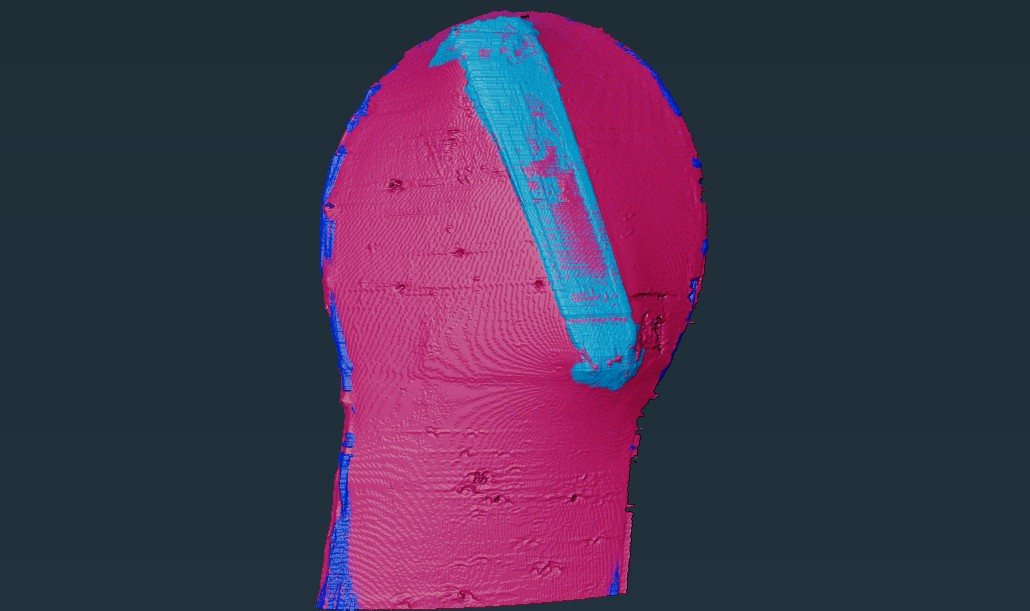
\includegraphics[width=0.5\textwidth]{images/avizo_flats/tlys2.jpg}
	\caption{text}
 \label{tlys2}
\end{figure}
\begin{figure}
	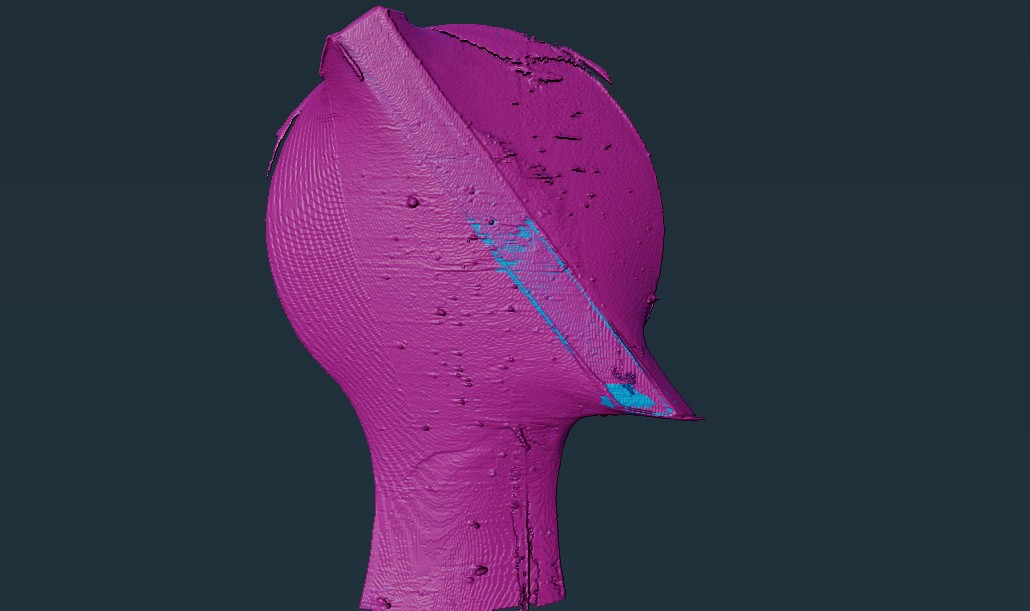
\includegraphics[width=0.5\textwidth]{images/avizo_flats/tlys_9.jpg}
	\caption{text}
 \label{tlys9}
\end{figure}
\begin{figure}
	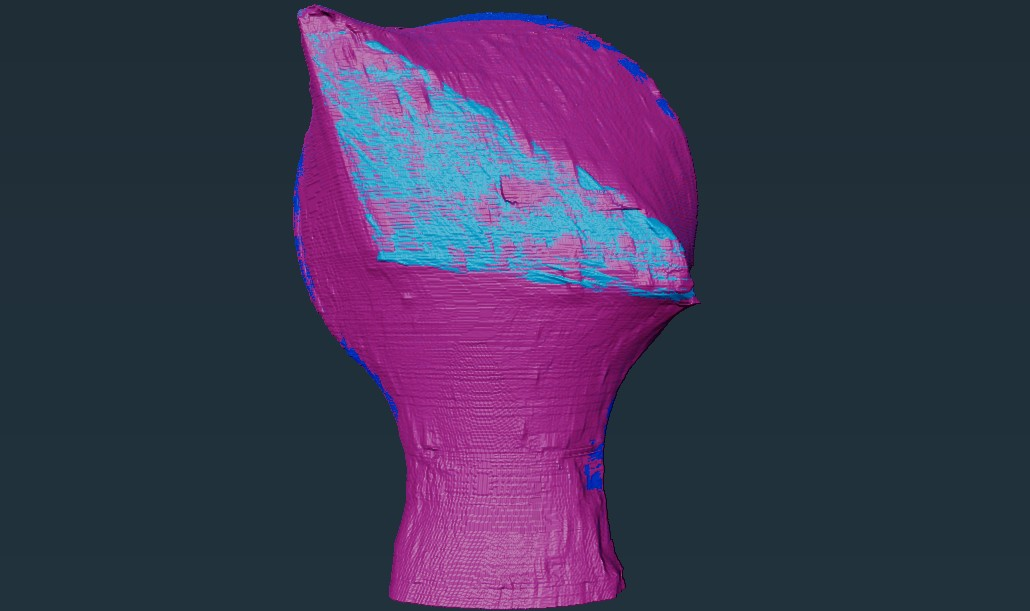
\includegraphics[width=0.5\textwidth]{images/avizo_flats/cas3_1118.jpg}
	\caption{text}
 \label{cas3}
\end{figure}



\begin{figure}
	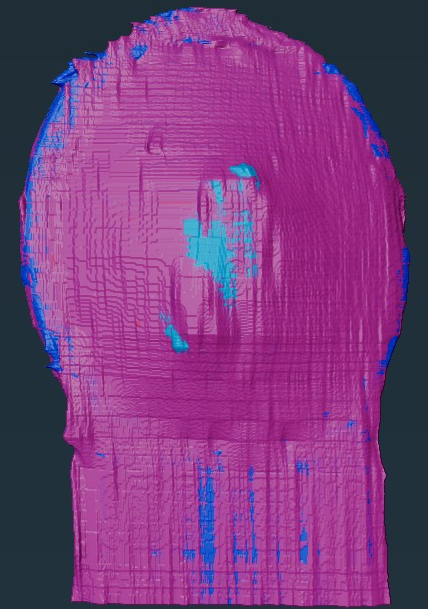
\includegraphics[width=0.5\textwidth]{images/avizo_flats/ins_con.jpg}
	\caption{text}
 \label{ins_control}
\end{figure}
\begin{figure}
	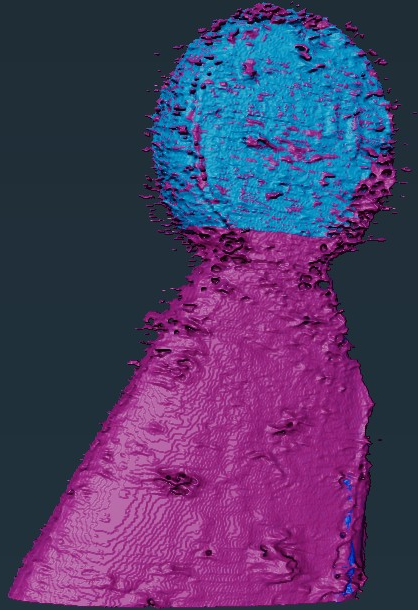
\includegraphics[width=0.5\textwidth]{images/avizo_flats/ins_ls.jpg}
	\caption{Laser-shaped insulin crystal}
 \label{ins_lasershaped}
\end{figure}

\begin{figure}
	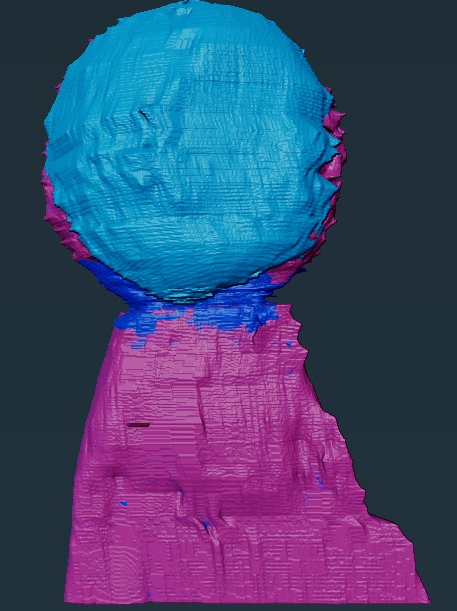
\includegraphics[width=0.5\textwidth]{images/avizo_flats/prot_ls.jpg}
	\caption{text}
\end{figure}
\begin{figure}
	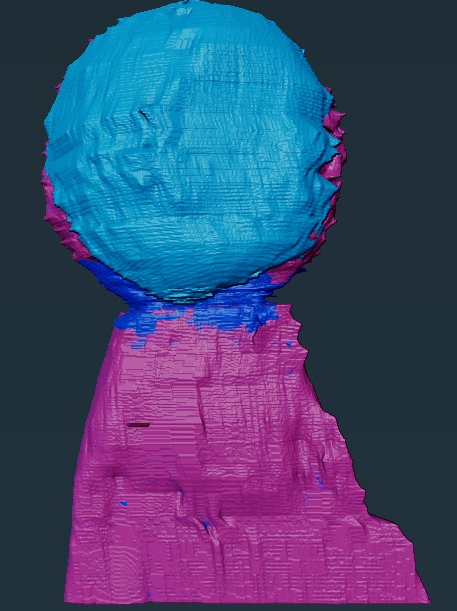
\includegraphics[width=0.5\textwidth]{images/avizo_flats/prot_ls.jpg}
	\caption{text}
\end{figure}


\onecolumn
\begin{figure}
	\centering
	\includegraphics{./plots/1.2_all_orders.pdf}
\end{figure}
\begin{figure}
	\includegraphics{./plots/1.2_orderpermute.pdf}
\end{figure}
\begin{figure}
	\centering
	\includegraphics[width=\textwidth]{./plots/fourfluxes.pdf}
\end{figure}
\begin{figure}
	\includegraphics{fourpurities.pdf}
\end{figure}
\begin{figure}
	\includegraphics{purityheatmap.pdf}
\end{figure}